\section{Evaluation}
\label{section::evaluation}

Our evaluation demonstrates the effectiveness of shuffled topologies and \PowerRouting at reducing the required capital investment in power infrastructure to meet a high-availability data center's reliability and power needs.  First, we demonstrate how shuffled topologies reduce the reserve capacity required to provide single-PDU-fault tolerance.  Then, we examine the effectiveness of \PowerRouting at further reducing provisioning requirements as a function of topology, number of PDUs, and workload.  Finally, we show how \PowerRouting will increase in effectiveness as server power management becomes more sophisticated and the gap between servers' idle and peak power demands grows.

\subsection{Methodology}
\label{section::methodology}

We evaluate \PowerRouting through analysis of utilization traces from a large collection of production systems. We simulate \PowerRouting's scheduling algorithm and impact on performance throttling and capital cost.

{\bf Traces.}
We collect utilization traces from three production facilities: (1) \emph{EECS servers}, a small cluster of departmental servers (web, email, login, etc.) operated by the Michigan EECS IT staff; (2) \emph{Arbor Lakes Data Center}, a ~1.5MW facility supporting the clinical operations of the University of Michigan Medical Center; and (3) \emph{Michigan Academic Computer Center (MACC)}, a 4MW high-performance computing facility operated jointly by the University of Michigan, Internet2, and Merit that runs primarily batch processing jobs.  These sources provide a diverse mix of real-world utilization behavior.  Each of the traces ranges in length from three to forty days sampling server utilization once per minute.  We use these traces to construct a hypothetical high-availability hosting facility  comprising 400 medical center servers, 300 high performance computing nodes, and a 300-node web search cluster.   The simulated medical center and HPC cluster nodes each replay a trace from a specific machine in the corresponding real-world facility.  The medical center systems tend to be lightly loaded, with one daily utilization spike (which we believe to be daily backup processing).  The HPC systems are heavily loaded.  As we do not have access to an actual 300-node web search cluster, we construct a cluster by replicating the utilization trace of a single production web server over 300 machines.  The key property of this synthetic search cluster is that the utilization on individual machines rises and falls together in response to user traffic, mimicking the behavior reported for actual search clusters \cite{Fan07}.  We analyze traces for a 24-hour period. Our synthetic cluster sees a time-average power draw of 180.5 kW, with a maximum of 208.7 kW and standard deviation of 9 kW.

{\bf Power.}  We convert utilization traces to power budget requests using published SPECPower results \cite{SpecPower}.  Most of our traces have been collected from systems where no SPECPower result has been published; for these, we attempt to find the closest match based on vendor descriptions and the number and model of CPUs and installed memory. As SPECPower only provides power at intervals of 10\% utilization, we use linear interpolation to approximate power draw in between these points.

Prior work \cite{Fan07,Ranganathan06} has established that minute-grained CPU utilization traces can predict server-grain power 
draw to within a few percent.   Because of the scope of our data collection efforts, finer-grained data collection is impractical.  Our estimates of savings from Power Routing are conservative; finer-grained scheduling might allow tighter tracking of instantaneous demand.  

To test our simulation approach, we have validated simulation-derived power values against measurements of individual servers in our lab.    Unfortunately, the utilization and power traces available from our production facilities are not exhaustive, which precludes a validation experiment where we compare simulation-derived results to measurements for an entire data center.
 
{\bf Generating data center topologies.} For each power distribution topology described in Section~\ref{section::intermixed}, we design a layout of our hypothetical facility to mimic the typical practices seen in the actual facilities. We design layouts according to the policies the Michigan Medical Center IT staff use to manage their \emph{Arbor Lakes} facility. Each layout determines an assignment of physical connections from PDUs to servers. Servers that execute similar applications are collocated in the same rack, and, hence, in conventional power delivery topologies, are connected to the same PDU.  Where available, we use information about the actual placement of servers in racks to guide our placement.  Within a rack, servers are assigned across PDU phases in a round-robin fashion.  We attempt to balance racks across PDUs and servers within racks across AC phases based on the corresponding system's power draw at 100\% utilization.  No server is connected to two phases of the same PDU, as this arrangement does not protect against PDU failure.  We use six PDUs in all topologies unless otherwise noted.

{\bf Metrics.} We evaluate \PowerRouting based on its impact on server throttling activity and data center capital costs.  As the effect of voltage and frequency scaling on performance varies by application, we instead use the fraction of requested server power budget that was not satisfied as a measure of the performance of capping techniques.  Under this metric, the ``cost" of failing to supply a watt of requested power is uniform over all servers, obviating the need to evaluate complex performance-aware throttling mechanisms (which are orthogonal to \PowerRouting). Our primary evaluation metric is the minimum total power delivery capacity required to assure zero performance throttling, as this best illustrates the advantage of \PowerRouting over conventional worst-case provisioning.

\subsection{Impact of Shuffled Topologies}

\begin{figure}[t!]
\centering
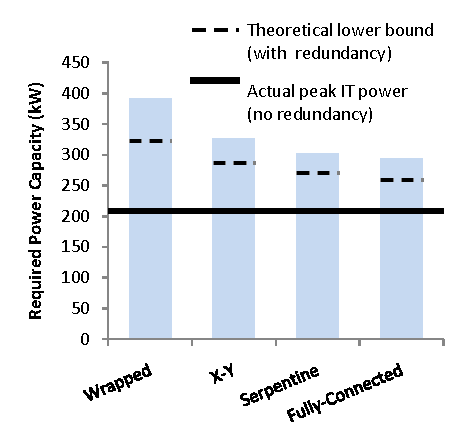
\includegraphics[width = 3.0 in]{Appendices/PowerRouting/figure/result_intermix.eps}
\caption{ \textbf{Minimum capacity for redundant operation under shuffled topologies (no Power Routing).} }
\label{figure::intermix}
\vspace{-.1 in}
\end{figure}

We first compare the impact of shuffled topologies on required power infrastructure capacity.  Shuffled topologies reduce the reserve capacity that each PDU must sustain to provide fault tolerance against single-PDU failure.  We examine the advantage of several topologies relative to the baseline high-availability ``wrapped" data center topology, which requires each PDU to be over-provisioned by 50\% of its nominal load.  We report the total power capacity required to prevent throttling for our traces.  We assume that each PDU must maintain sufficient reserve capacity at all times to precisely support the time-varying load that might fail over to it.

Differences in the connectivity of the various topologies result in differing reserve capacity requirements.
For an ideal power distribution infrastructure (one in which load is perfectly balanced across all PDUs), each PDU must reserve $\frac{1}{c + 1}$ to support its share of a failing PDU's load, where $c$ is the \emph{fail-over connectivity} of the PDU.  Fail-over connectivity counts the number of distinct neighbors to which a PDU's servers will switch in the event of failure. It is two for the wrapped topology, four for serpentine, and varies as a function of the number of PDUs for X-Y and fully-connected topologies. As the connectivity increases, reserve requirements decrease, but with diminishing returns.

To quantify the impact of shuffled topologies, we design an experiment where we statically assign each server the best possible primary and secondary power feed under the constraints of the topology.  We balance the average power draw on each PDU using each server's average power requirement over the course of the trace. (We assume this average to be known a priori for each server.)  

In Figure~\ref{figure::intermix} each bar indicates the required power capacity for each topology to meet its load and reserve requirements in all time epochs  (i.e., no performance throttling or loss of redundancy) for a 6 PDU data center.  For 6 PDUs, the fail-over connectivities are 2, 3, 4, and 5 for the wrapped, X-Y, serpentine, and fully-connected topologies, respectively.  The dashed line on each bar indicates the topology's theoretical lower-bound capacity requirement to maintain redundancy if server power draw could be split dynamically and fractionally across primary and secondary PDUs (which \PowerRouting approximates).  The gap between the top of each bar and the dashed line arises because of the time-varying load on each server, which creates imbalance across PDUs and forces over-provisioning. The solid line crossing all bars indicates the data center's peak power draw, ignoring redundancy requirements (i.e., the actual peak power supplied to IT equipment).

Topologies with higher connectivity require less reserve capacity, though the savings taper off rapidly.  The X-Y and serpentine topologies yield impressive savings and are viable and scalable from an implementation perspective.  Nevertheless, there is a significant gap between the theoretical (dashed) and practical (bar) effectiveness of shuffled topologies.  As we show next, \PowerRouting closes this gap.   

\subsection{Impact of \PowerRouting}
\label{sec::routing}

{\bf \PowerRouting effectiveness.}
To fully explore \PowerRouting effectiveness, we repeated the analysis above for all four topologies (wrapped, X-Y, serpentine, and fully-connected) and contrast the capacity required to avoid throttling for each. For comparison, we also reproduce the capacity requirements without \PowerRouting (from Figure~\ref{figure::intermix}).  We show results in Figure~\ref{figure::powerrouting}.
Again, a dashed line represents the theoretical minimum capacity necessary to maintain single-PDU fault redundancy for our workload and the given topology; the solid line marks the actual peak IT power draw. Because the overall load variation in our facilities is relatively small (HPC workloads remain pegged at near-peak utilization; the medical facility is over-provisioned to avoid overloading), we expect a limited opportunity for \PowerRouting.  Nonetheless, we reduce required power delivery capacity for all topologies (except wrapped) by an average of 12\%.

From the figure, we see that the sparsely-connected wrapped topology is too constrained for \PowerRouting to be effective; \PowerRouting requires 20\% more than the theoretical lower bound infrastructure under this topology. The three shuffled topologies, however, nearly reach their theoretical potential, even with a heuristic scheduling algorithm.
Under the fully-connected topology, \PowerRouting comes within 2\% of the bound, reducing power infrastructure requirements by over 39kW (13\%) relative to the same topology without \PowerRouting and more than 35\% relative to the baseline wrapped topology without \PowerRouting.
Our result indicates that more-connected topologies offer an advantage to \PowerRouting by providing more freedom to route power.
However, the the more-practical topologies yield similar infrastructure savings; the serpentine topology achieves 32\% savings relative to the baseline.

\begin{figure}[t!]
\centering
\includegraphics[width = 3.0 in]{Appendices/PowerRouting/figure/result_powerrouting.eps}
\caption{ \textbf{\PowerRouting infrastructure savings as a function of topology.} }
\label{figure::powerrouting}
\vspace{-.1 in}
\end{figure}

{\bf Sensitivity to number of PDUs.}
The number of PDUs affects \PowerRouting effectiveness, particularly for the fully-connected topology. Figure~\ref{figure::pdus} shows this sensitivity for four to eight PDUs. For a fixed total power demand, as the number of PDUs increases, each individual PDU powers fewer servers and requires less capacity.  With fewer servers, the variance in power demands seen by each PDU grows (i.e., statistical averaging over the servers is lessened), and it becomes more likely that an individual PDU will overload. Without \PowerRouting, this effect dominates, and we see an increase in required infrastructure capacity as the number of PDUs increases beyond 6.  At the same time, increasing the number of PDUs offers greater connectivity for certain topologies, which in turn lowers the required slack that PDUs must reserve and offers \PowerRouting more choices as to where to route power.  Hence, \PowerRouting is better able to track the theoretical bound and the required power capacity decreases with more PDUs.


\begin{figure}[t!]
\centering
\includegraphics[width = 3.0 in]{Appendices/PowerRouting/figure/result_numPDUs.eps}
\caption{ \textbf{Sensitivity of the fully-connected topology to number of PDUs.} }
\label{figure::pdus}
\vspace{-.1 in}
\end{figure}

\subsection{\PowerRouting For Low Variance Workloads}
%{\bf \PowerRouting for low variance workloads.}
The mixed data center trace we study is representative of the diversity typical in most data centers.  Nevertheless, some data centers run only a single workload on a homogeneous cluster.  \PowerRouting exploits diversity in utilization patterns to shift power delivery slack; hence, its effectiveness is lower in homogeneous clusters.  

\begin{figure*}[t]
\centering
\subfigure[Arbor Lakes (clinical operations)]{
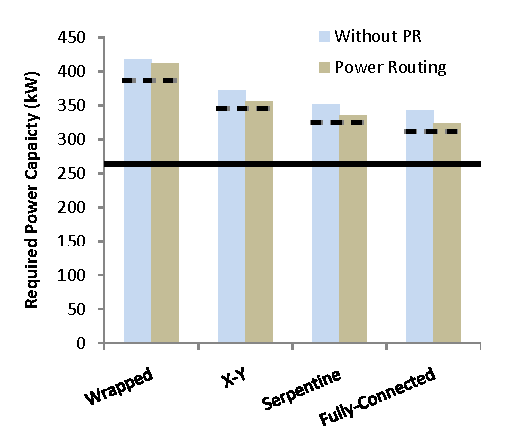
\includegraphics[width=3.0 in]{Appendices/PowerRouting/figure/result_AL.eps}
\label{figure::AL}
}
\hspace{0.5in}
\subfigure[MACC (high-performance computing)]{
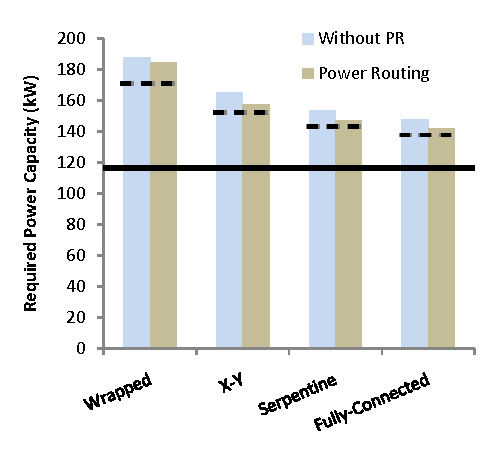
\includegraphics[width=3.0 in]{Appendices/PowerRouting/figure/result_nyx.eps}
\label{figure::nyx}
}
\vspace{-0.15 in}
\caption{ \textbf{\PowerRouting effectiveness in homogeneous data centers.} }
\vspace{-0.15 in}
\label{figure::homogenous}
\end{figure*}

To explore these effects, we construct \PowerRouting test cases for 1000-server synthetic clusters where each server runs the same application.  We do not study the web search application in isolation; in this application, the utilization on all servers rise and fall together, hence, the load on all PDUs is inherently balanced and there is no opportunity (nor need) for \PowerRouting. Instead, we evaluate \PowerRouting using the medical center traces and high performance computing traces, shown in Figures~\ref{figure::AL} and \ref{figure::nyx}, respectively. 

The high performance computing cluster consumes a time-average power of 114.9 kW, a maximum of 116.4 kW, and a standard deviation of 0.8 kW while the medical center computing traces consume a time-average power of 254.6 kW, with maximum 263.6 kW and standard deviation 2.4 kW.  In both cases, the variability is substantially lower than in the heterogeneous data center test case.

Although \PowerRouting comes close to achieving the theoretical lower bound infrastructure requirement in each case, we see that there is only limited room to improve upon the non-\PowerRouting case. Even the baseline wrapped topology requires infrastructure that exceeds the theoretical bound by only 7.5\% for the high performance computing cluster and 5\% for the medical data center. We conclude that \PowerRouting offers substantial improvement only in heterogeneous clusters and applications that see power imbalance, a common case in many facilities.

\subsection{\PowerRouting With Energy-Proportional Servers}
%{\bf \PowerRouting with Energy-Proportional Servers.}
As the gap between servers' peak and idle power demands grows  (e.g., with the advent of energy-proportional computers \cite{Barroso07}), we expect the potential for \PowerRouting to grow. The increase in power variance leads to a greater imbalance in power across PDUs, increasing the importance of correcting this imbalance with \PowerRouting.

To evaluate this future opportunity, we perform an experiment where we assume all servers are energy-proportional---that is, servers whose power draw varies linearly with utilization---with an idle power of just 10\% of peak.  This experiment models servers equipped with PowerNap \cite{Meisner09}, which allows servers to sleep during the millisecond-scale idle periods between task arrivals.  We repeat the experiment shown in Figure~\ref{figure::powerrouting} under this revised server power model. The results are shown in Figure~\ref{figure::powernap}.  Under these assumptions, our traces exhibit a time-average power of 99.8 kW, maximum of 153.9 kW, and standard deviation of 18.9 kW.

\PowerRouting is substantially more effective when applied to energy-proportional servers. 
However, the limitations of the wrapped topology are even more pronounced in this case, and \PowerRouting provides little improvement. Under the more-connected topologies, \PowerRouting is highly effective, yielding reductions of 22\%, 29\%, and 28\% for the X-Y, serpentine, and fully-connected topologies, respectively, relative to their counterparts without \PowerRouting.
As before, the more-connected topologies track their theoretical lower bounds more tightly.  Relative to the baseline wrapped topology, a serpentine topology with \PowerRouting yields a 47\% reduction in required physical infrastructure capacity. It is likely that as computers become more energy-proportional, power infrastructure utilization will continue to decline due to power imbalances.
\PowerRouting reclaims much of this wasted capacity.

\begin{figure}[t!]
\centering
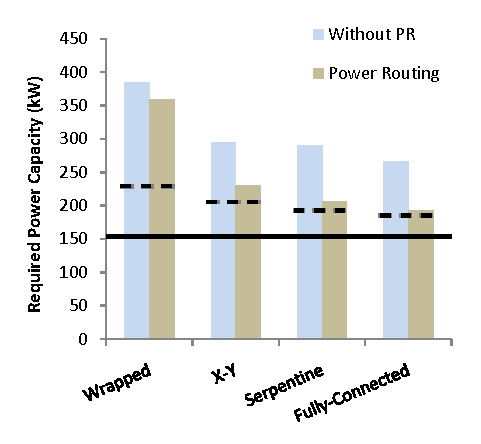
\includegraphics[width = 3.0 in]{Appendices/PowerRouting/figure/result_powernap.eps}
\vspace{-.1 in}
\caption{ \textbf{Impact with energy-proportional servers.} }
\label{figure::powernap}
\vspace{-.15 in}
\end{figure}


\subsection{Limitations}

Our evaluation considers workloads in which any server may be throttled, and our mechanisms make no effort to select servers for throttling based on any factors except maximizing the utilization of the power delivery infrastructure.  In some data centers, it may be unacceptable to throttle performance.  These data centers cannot gain a capital cost savings from under-provisioning; their power infrastructure must be provisioned for worst case load.  Nonetheless, these facilities can benefit from intermixed topologies (to reduce reserve capacity for fault tolerance) and from the phase-balancing possible with \PowerRouting.
